\documentclass{standalone}
\usepackage{tikz}
\begin{document}
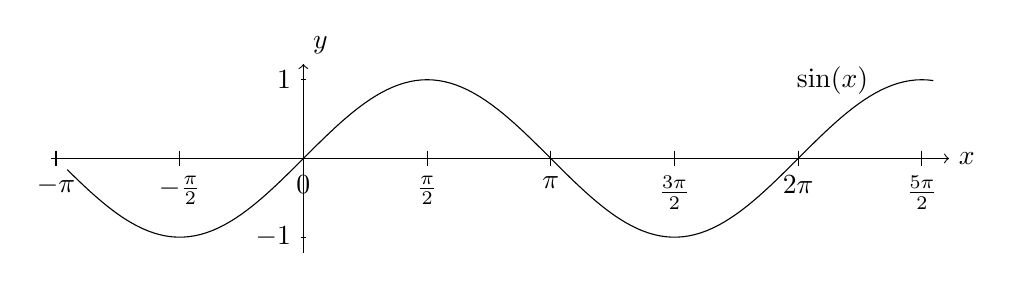
\begin{tikzpicture}[domain=-3:8]
    \draw[->] (-3.2,0) -- (8.2,0) node[right] {$x$};
    \draw[->] (0,-1.2) -- (0,1.2) node[anchor=south west] {$y$};
    \draw plot [samples=150] (\x,{sin(\x r)})  node[right, anchor=east] {$ \sin (x)$\qquad\qquad};
    \foreach \x/\xtext in {-pi/-\pi, -0.5*pi/-\frac{\pi}{2}, 0,0.5*pi/\frac{\pi}{2}, pi/\pi, 1.5*pi/\frac{3\pi}{2}, 2*pi/2\pi, 2.5*pi/\frac{5\pi}{2} }
      \draw (\x,0.1) -- (\x,-0.1) node[anchor=north] {$\xtext$};
     \foreach \y/\ytext in {-1,1}
       \draw (1pt,\y cm) -- (-1pt,\y cm) node[anchor=east] {$\ytext$};
\end{tikzpicture}


 \end{document}
